\documentclass{article}
\usepackage[utf8]{inputenc}
\usepackage{polski}

\usepackage{bbm}
\usepackage{graphicx}    
\usepackage{caption}
\usepackage{subcaption}
\usepackage{epstopdf}
\usepackage{amsmath,amssymb,amsfonts,amsthm,mathtools}
\usepackage{hyperref}
\usepackage{url}
\usepackage{comment}
\usepackage[section]{placeins}
\newtheorem{defi}{Definicja}
\newtheorem{twr}{Twierdzenie}


\author{Jan Mazur 281141}
\date{Wrocław, \today}
\title{\textbf{Obliczanie wartośći funkcji $\textrm{arctan}$ i $\textrm{arccot}$ } \\ Sprawozdanie do zadania P.1.4}

\begin{document}
\maketitle

\section{Wstęp}

Zadanie polega na obliczaniu wartośći funkcji $f(x) = \arctan(x)$ oraz\\ $f(x) = \textrm{arccot}(x)$, przy wykorzystaniu jedynie podstawowych działań arytmetycznych ( $+$, $-$, $*$, $/$ ).

\indent Przedstawię różne sposoby obliczania wartości tych funkcji - szereg Taylora, szereg Eulera oraz nieskończony ułamek łańcuchowy. 
Dokładność wszystkich metod porównam z funkcjami biblioteczymi.
Wartośći funkcji  $\textrm{arccot}(x)$ będę wyliczał za pomocą wzorów matematycznych używając wcześniej wyliczonej wartośći funkcji $\arctan(x)$.

%\indent Za wyznacznik dokładności metod przyjąłem ilość dokładnych cyfr znaczących obliczonej wartości w stosunku do wartości obliczonej za pomocą funkcji bibliotecznej.

\indent Wszelkie obliczenia wykonane zostały przy użyciu języka programowania \textbf{Julia} w wersji \textbf{0.5.0}, symulując 1000-bitową mantysę zmiennopozycjnego zapisu liczb maszynowych.

\indent Kod źródłowy który został użyty do obliczeń, oraz do generowania wykresów znajduje się w pliku o rozszerzeniu .ipynb

\section{Uwarunkowanie zadania}
Przed przystąpieniem do jakichkolwiek obliczeń sprawdzam uwarunkowanie zadania. Wyznaczam wskaźniki urarunkowania obliczania wartości obu funkcji:
\begin{equation*}{\displaystyle cond(\mathbf {\arctan}(x) )}=\frac{x}{\left ( 1+x^{2} \right )\arctan (x)}\end{equation*}
\begin{equation*}
{\displaystyle cond(\mathbf {\arccot}(x) )}=\frac{x}{\left ( 1+x^{2} \right )\arccot (x)}
\end{equation*}


\indent Po prostej analizie obu funkcji dostajemy własności:
\begin{equation*}
{\displaystyle cond(\mathbf {\arctan}(x) )} \leq 1
\end{equation*}
\begin{equation*}
{\displaystyle cond(\mathbf {\arccot}(x) )} \leq 1
\end{equation*}

Oba wskaźniki uwarunkowania są ograniczone przez niewielką stałą, więc zadanie jest dobrze uwarunkowane. 

\section{Szereg Taylora}
Pierwszy sposób obliczania wartości funkcji $\arctan(x)$ opiera się o rozwinięcie jej w szereg Taylora \cite{fichtenholz}

\begin{equation}
\arctan(x)=x-{\frac {x^{3}}{3}}+{\frac {x^{5}}{5}}-{\frac {x^{7}}{7}}+\cdots =\sum _{n=0}^{\infty }{\frac {(-1)^{n}x^{2n+1}}{2n+1}}\,;\qquad |x|\leq 1\qquad 
\end{equation}

Algorytm oblicza n-tą sumę częściową powyższego szeregu.\\
Szereg ten jest zbieżny tylko dla $x \in [-1,1]$, a funkcja $\arctan(x)$ określona jest dla wszystkich rzeczywistych $x$.
Problem ten rozwiążemy w punkcie 6.

\begin{table}[h]
	\centering
	\begin{tabular}{|c|c|} \hline
		n-ta suma częściowa & błąd bezwzględny \\ \hline
		1 &  3.63e-02\\
		2 &  5.31e-03\\
		3 &  9.35e-04\\
		4 &  1.80e-04\\
		5 &  3.66e-05\\
		\vdots & \vdots \\
		30  &  5.72e-21 \\
		40 &  4.10e-27 \\
		50 &  3.13e-33\\
		\hline
	\end{tabular}
	\caption{Błędy bezwzględne przy obliczaniu kolejnych sum częściowych w punkcie $x = 0.5$}
\end{table}

\section{Szereg Eulera}

Funkcję $\arctan(x)$ wyrazić można również za pomocą innego szeregu - szeregu Eulera \cite{wolfram}:

\begin{equation}
\arctan (x)=\sum _{n=0}^{\infty }{\frac {2^{2n}(n!)^{2}}{(2n+1)!}}\;{\frac {x^{2n+1}}{(1+x^{2})^{n+1}}}
\end{equation}

W tym przypadku algorytm również liczy n-tą sumę częściową szeregu.\\
Z kryterium d'Alemberta ten szereg jest zbieżny dla wszystkich $x \in \mathbb{R} $.\\
Szereg ten zbiega nieznacznie szybciej niż szereg opisany w punkcie 3.

\begin{table}[h]
	\centering
	\begin{tabular}{|c|c|} \hline
		n-ta suma częściowa & błąd bezwzględny \\ \hline
		1 &  6.36e-02\\
		2 &  1.03e-02\\
		3 &  1.78e-03\\
		4 &  3.18e-04\\
		5 &  5.80e-05\\
		\vdots & \vdots \\
		30  &  8.54e-23 \\
		40 &  7.60e-30 \\
		50 &  6.98e-37\\
		\hline
	\end{tabular}
	\caption{Błędy bezwzględne przy obliczaniu kolejnych sum częściowych w punkcie $x = 0.5$}
\end{table}

\section{Nieskończony ułamek łańcuchowy}
Funkcja $\arctan$ może zostać zapisana również za pomocą nieskończonego ułamka łańcuchowego \cite{wolfram}\cite{deutsch}:

\begin{equation}
\arctan(x)={\frac {x}{1+{\cfrac {(1x)^{2}}{3+{\cfrac {(2x)^{2}}{5+{\cfrac {(3x)^{2}}{7+{\cfrac {(4x)^{2}}{9+\ddots }}}}}}}}}}
\end{equation}

Dany ułamek jest zbieżny dla wszystkich $x \in \mathbb{R} $.\\
Algorytm oblicza ułamek do zadanego n-tego reduktu. 
Metoda ta okazuje się być najszybciej zbieżna ze wszystkich przeze mnie analizowanych.

\begin{table}[h]
	\centering
	\begin{tabular}{|c|c|} \hline
		n-ty redukt & błąd bezwzględny \\ \hline
		1 &  1.56e+00\\
		2 &  2.10e-03\\
		3 &  1.20e-04\\
		4 &  6.80e-06\\
		5 &  3.82e-07\\
		\vdots & \vdots \\
		30  &  1.77e-38 \\
		40 &  5.13e-51 \\
		50 &  1.48e-63\\
		\hline
	\end{tabular}
	\caption{Błędy bezwzględne przy obliczaniu kolejnych reduktów ułamka dla $x = 0.5$}
\end{table}

\section{Redukcja argumentu}

Opisane przeze mnie metody są dobrze zbieżnie w przedziale $[-1,1]$, natomiast poza tym przedziałem są zbieżne dużo wolniej, albo nawet wcale.
Aby zaradzić temu problemowi skorzystałem ze wzoru \cite{wiki}:

\begin{equation}
	{\begin{aligned}\arctan(x)&=2\arctan \left({\frac {x}{1+{\sqrt {1+x^{2}}}}}\right)\end{aligned}}
\end{equation}

Co prawda wymaga on obliczania pierwiastka, czego treść zadania nie dopuszcza, jednakże prostym algorytmem obliczania pierwiastka zgodnym z treścią zadania jest metoda babilońska \cite{babylon}, którą pozwolę sobię pominąć.
\linebreak

Funkcja w argumencie $\arctan(x)$ po prawej stronie równości ma zbiór wartości równy $(-1,1)$, zatem wystarczy przed obliczeniami raz skorzystać z tego wzoru, aby znaleźć się w przedziale zbieżności opisanych metod.
Doświadczenia numeryczne pokazują jednak, że opłaca się zmniejszyć argument jak najbardziej, czyli skorzystać z tego wzoru kilkukrotnie, redukując argument do określonej z góry wartości. Można zaobserwować to na wykresach w punkcie 8 jako "skoki" wykresu.

\section{Obliczanie arccot(x)}
W celu obliczenia wartośći funkcji $\textrm{arccot}(x)$ skorystam ze wzoru \cite{wiki}:

\begin{equation}
\arctan \left({\frac {1}{x}}\right)=\operatorname {arccot}(x)
\end{equation}

\noindent
Do obliczenia $\arctan(\frac{1}{x})$ użyję opisanych wcześniej metod.

\clearpage
\section{Porównanie zbieżności metod}

Używam słowa "iteracja" mając na myśli krok algorytmu. W przypadku szeregów jest to policzenie kolejnej sumy częściowej a w przypadku ułamka łańcuchowego, policzenie ułamka z jednym reduktem więcej.

\subsection{Dla funkcji arctan(x)}

	\begin{figure}[h]
		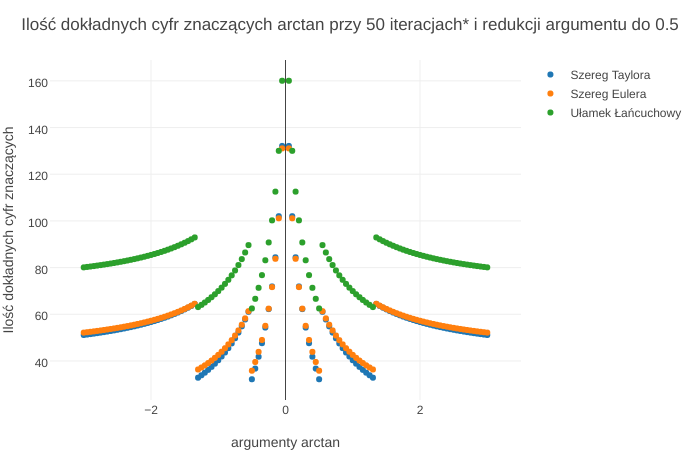
\includegraphics[width=1.1\textwidth,scale=1]{atan_znaczace.png}
		\caption{porownanie ilości dokładnych cyfr znaczących}
		\label{wskaźnik uwarunkowania}
	\end{figure}
\FloatBarrier
\noindent Na wykresie widać, że metoda obliczania wartości funkcji $\arctan(x)$ za pomocą ułamka łańcuchowego daje zdecydowanie lepszą dokładność niż metody wykorzystujące szeregi. Dla argumentów blisko zera metoda wykorzystująca szereg Taylora jest nieznacznie lepsza niż metoda wykorzystująca rozwinięcie w szereg Eulera. W każdym innym miejscu okazuje się ona być najgorszą metodą. Dla coraz bardziej odległych od zera argumentów, metody są coraz gorzej zbieżne.

\indent "Skoki" wwykresu w obrębie jednego koloru związane są z redukcją argumentu. Obliczamy wtedy wartość funkcji dla argumentu, dla którego metoda jest zbieżna dużo szybciej.

\pagebreak
\subsection{Dla funkcji arccot(x)}
	\FloatBarrier
	\begin{figure}[h]
		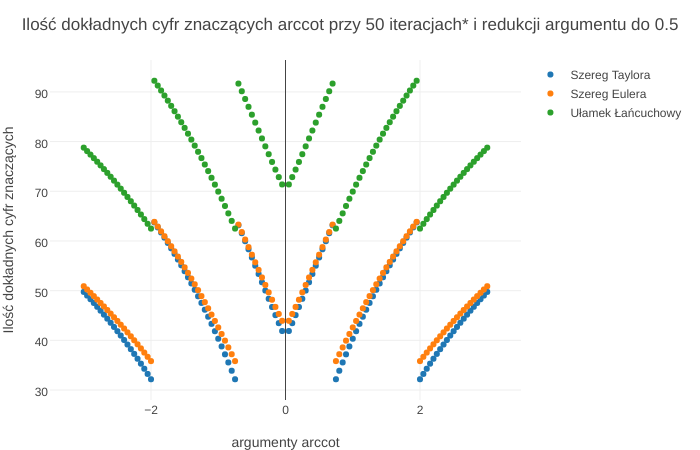
\includegraphics[width=1.1\textwidth,scale=0.5]{acot_znaczace.png}
		\caption{porownanie ilości dokładnych cyfr znaczących}
		\label{wskaźnik uwarunkowania}
	\end{figure}

Na tym wykresie zaobserwować możemy analogiczne rzeczy co na wykresie powyżej. Analogia wynika z liczenia odwrotności argumentu $\textrm{arccot}$ jako argument $\arctan$. W tym przypadku szybkość zbieżności metod rośnie wraz ze wzrostem odległości argumentu od zera.
	
\section{Wnioski}
Po rozważeniu 3 różnych metod obliczania wartości podanych w zadaniu funkcji stwierdzam, iż najlepszą metodą jest metoda wykorzystująca postać nieskończonego ułamka łańcuchowego. Wzór ten jest prawdziwy dla wszystkich argumentów funkcji a ponadto zbiega dużo szybciej niż pozostałe metody.\\
\indent Dodatkowo bardzo opłacalną operacją jest redukcja argumentu dla którego liczymy wartość funkcji.


\begin{thebibliography}{9}
	\itemsep2pt
	
		\bibitem{deutsch} Oskar Perron - "Die Lehre von den Kettenbrüchen"
		
		\bibitem{fichtenholz} G. R Fichtenholz - "Rachunek różniczkowy i całkowy" - tom I, rodział III, paragraf 5
	\bibitem{taylor} Weisstein, Eric W. "Euler's Continued Fraction." From MathWorld--A Wolfram Web Resource. \url{http://mathworld.wolfram.com/EulersContinuedFraction.html}
	(ostatni dostęp \today)
	
%%	\bibitem{fraction} \url{http://mathworld.wolfram.com/e.html}
%%	(ostatni dostęp \today).
	
	\bibitem{wolfram}
	Weisstein, Eric W. "Inverse Tangent." From MathWorld--A Wolfram Web Resource.\url{http://mathworld.wolfram.com/InverseTangent.html} 
	(ostatni dostęp \today)
	 
	
	\bibitem{wiki} \url{https://en.wikipedia.org/wiki/Inverse_trigonometric_functions}
	(ostatni dostęp \today)
	
	\bibitem{babylon}
	\url{https://en.wikipedia.org/wiki/Methods_of_computing_square_roots}
	(ostatni dostęp \today)
	
\end{thebibliography}

\end{document}